\documentclass{article}
\usepackage{enumerate}
\usepackage[utf8]{inputenc}
\usepackage{graphicx}

\begin{document}

\begin{enumerate}[1)]
\item{% 1)
    \begin{enumerate}[a)]
    \item{% a)
        En una dimensión, y con las constantes dadas, el problema puede reescribirse como:

        \[ \frac{\partial^2 T}{\partial x^2} - T = -1 \]

        La solución analítica de esta ecuación diferencial es:

        \[ T(x) = A e^x + B e^{-x} + 1 \]

        Para obtener los valores de $A$ y de $B$ utilizamos las condiciones de contorno:

        \[ T(0) = A + B + 1 = 0 \Rightarrow B = -1 - A \]
        \begin{eqnarray*} 
            T(L) = A e^L + B e^{-L} + 1 &=& 1 \\
            \Rightarrow A e^L - e^{-L}  - A e^{-L} + 1 &=& 1 \\
            \Rightarrow A \left(e^L - e^{-L}\right) &=& e^{-L} \\
            \Rightarrow A  &=& \frac{e^{-L}}{e^L - e^{-L}} \\
            \Rightarrow B  &=& \frac{e^{L}}{e^{-L} - e^L} \\
        \end{eqnarray*}
    }
    \item{% b)
        Usando $L=1$:

        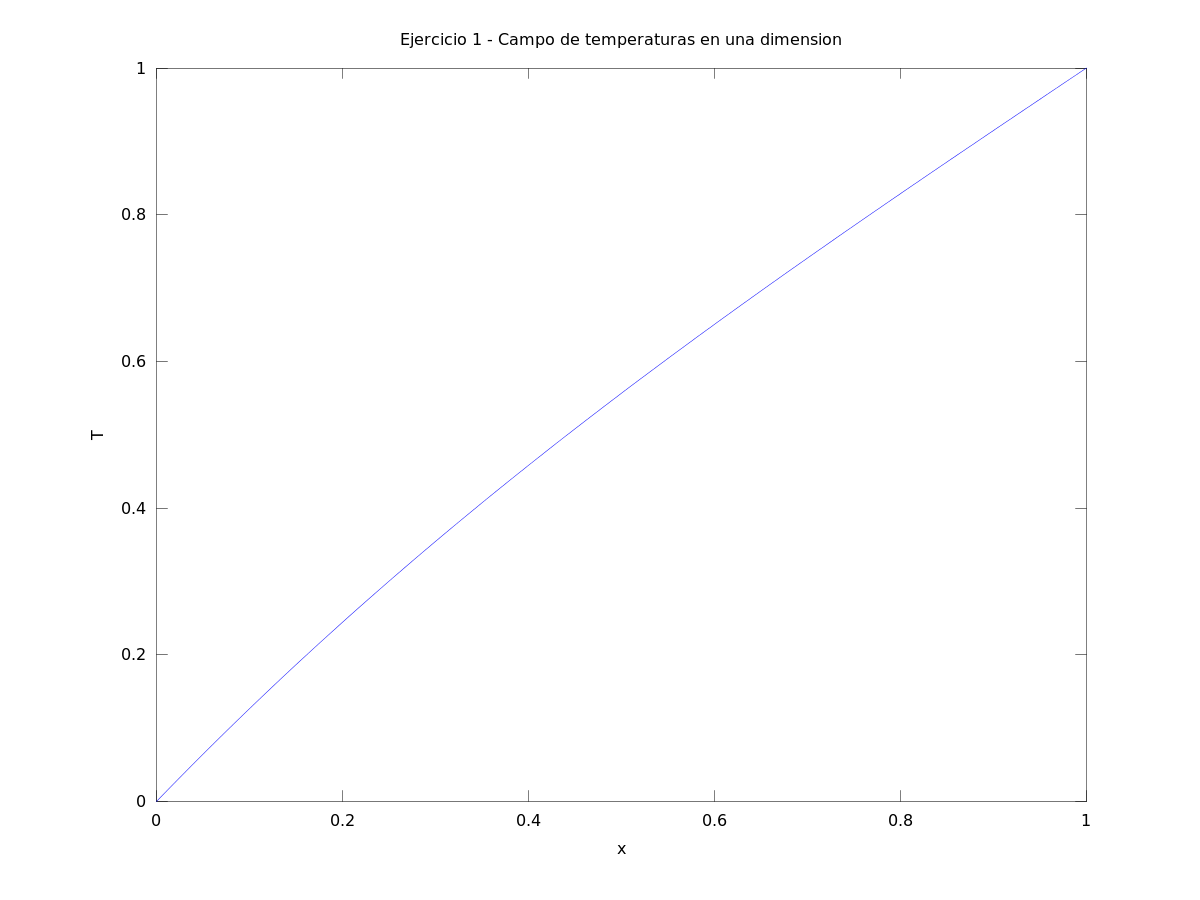
\includegraphics[width=\textwidth]{ej1_campo_temperatura.png}
    }
    \item{% c)
        Usamos la fórmula $q = -k \nabla T$ y obtenemos:

        \[ q(x) = -A e^x + B e^{-x} \]

        La gráfica para los valores dados es:

        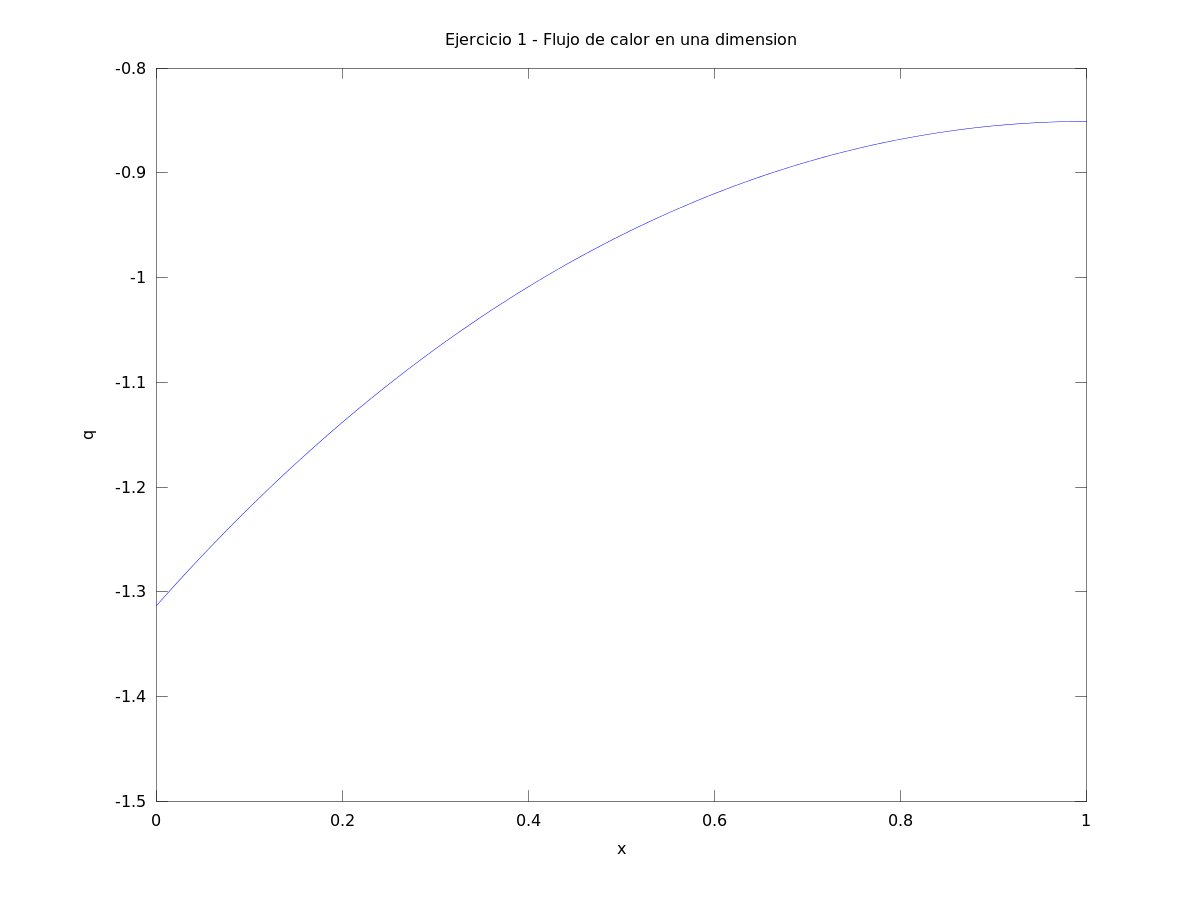
\includegraphics[width=\textwidth]{ej1_flujo_calor.png}

    }
    \end{enumerate}
}
\item{% 2)
    \begin{enumerate}[a)]
    \item{% a)
        El campo de temperaturas tiene la misma forma que el del ejercicio anterior:

        \[ T(x) = A e^x + B e^{-x} + 1 \]

        Y el flujo de calor es:

        \[ q(x) = B e^{-x} - A e^x \]

        Lo que cambia son las constantes:

        \begin{eqnarray*}
            A &=& - \frac{1+e^{-L}}{e^L + e^{-L}} \\
            B &=& - \frac{1-e^L}{e^L + e^{-L}}
        \end{eqnarray*}
    }
    \item{% b)
        Nuevamente usando $L=1$:

        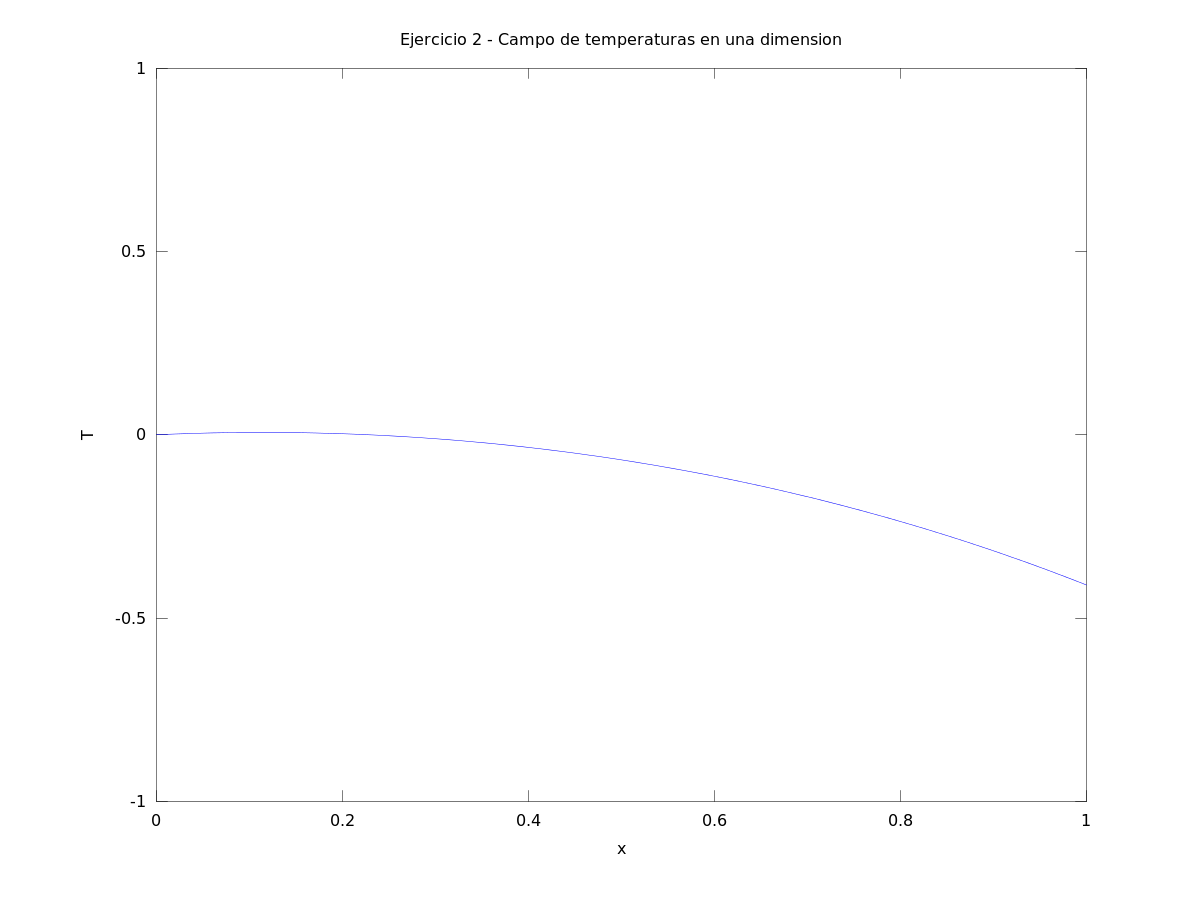
\includegraphics[width=\textwidth]{ej2_campo_temperatura.png}

    }
    \item{% c)
        \  

        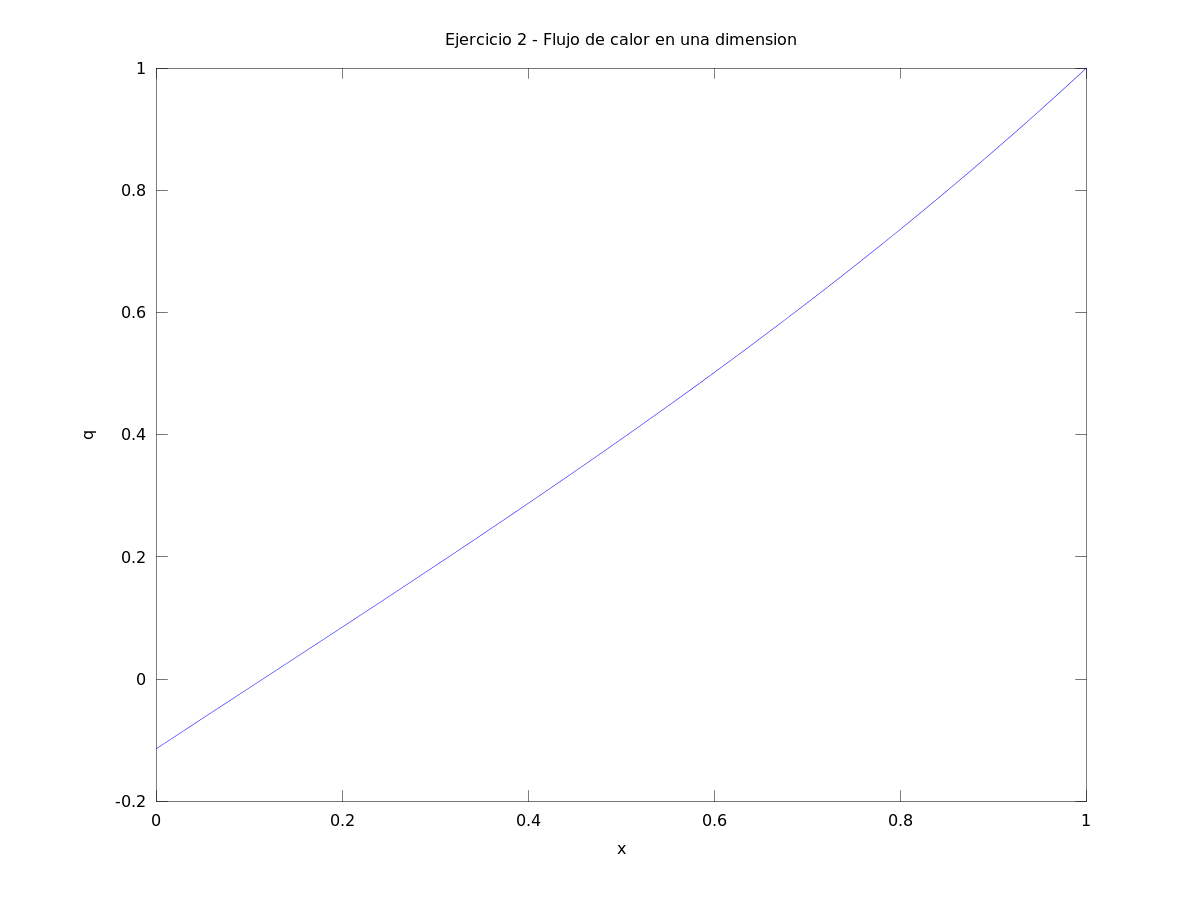
\includegraphics[width=\textwidth]{ej2_flujo_calor.png}
    }
    \end{enumerate}

}
\end{enumerate}

\end{document}
